\chapter{Projeto de estratégia de controle}
\label{controle}

Neste capítulo são detalhados os procedimentos necessários para implementação de estratégias de controle no ambiente de simulação. Inicialmente é descrita a organização e a estrutura dos arquivos necessários para implementação da estratégia de controle. Por fim, apresenta-se o processo de criação de uma nova estratégia de controle com a finalidade de ilustrar o procedimento apresentado na Seção \ref{SecEstCtrl}.

\section{Organização}

%O espaço de trabalho do ROS é organizado em módulos de software denominados "Pacotes". O ambiente de simulação, por sua vez, aproveita dessa organização para sistematizar o projeto de estratégia de controle, pois cada projeto é considerado um pacote. 

De modo geral a estrutura de arquivos do projeto de controle está organizada como illustrado na Figura \ref{pacote}:%, deve possuir os seguintes diretórios e arquivos: \\

\begin{figure}[H]
	\center
	\begin{tikzpicture}[%
	grow via three points={one child at (0.5,-0.7) and
		two children at (0.5,-0.7) and (0.5,-1.4)},
	edge from parent path={(\tikzparentnode.south) |- (\tikzchildnode.west)}]
	\node {Name\_of\_control\_Strategy/}
	child { node {src/}
		child { node {main.cpp}}
	}
	child [missing] {}
	child { node {include/}}		
	child { node {CMakeLists.txt}}
	child { node {package.xml}};
	\end{tikzpicture}
	\caption{Organização do diretório de projeto de estratégias de controle. Os diretórios são dados pelas ''caixinhas'' com nomes terminados pelo caractere ''/'' e os arquivos possuem alguma extensão em seu nome.}
	\label{pacote}
\end{figure}


%\noindent
%Obs.: Os diretórios são dados pelas ''caixinhas'' com nomes terminados pelo caractere ''/'', e os arquivos possuem alguma extensão em seu nome.


\begin{itemize}
	\itemsep0em 
	\item[-]O arquivo ''main.cpp'' é o arquivo onde é implementada a lógica da estratégia de controle.
	\item[-]A pasta ''include'' armazena bibliotecas customizadas pelo usuário que são incluídas no preâmbulo do arquivo main.cpp.
	\item[-]O arquivo ''CMakeLists.txt'' fornece ao compilador informações sobre o diretório de bibliotecas incluídas nos códigos fontes do simulador. Detalhes sobre como incluir novas bibliotecas podem ser encontrados no Apêndice \ref{cmake}.
	\item[-]O arquivo ''package.xml'' é o arquivo necessário para armazenar dados como nome do autor, endereço de e-mail, etc. Detalhes de sua configuração são apresentados no Apêndice \ref{package}.
\end{itemize}



\section{Interface padrão para desenvolvimento de estratégias de controle e template main.cpp}

A criação de uma estratégia de controle é realizada através de herança da classe virtual padrão "IController". Sendo essa uma classe virtual, seus métodos precisam ser implementadas na classe filha. A Figura \ref{interface} ilustra suas funções métodos. 

A função método  \textit{config()} é executada no inicio das simulações, sendo utilizada para realizar configurações iniciais da estratégia de controle. O método \textit{execute()} é chamado pelo simulador a cada período de amostragem. Ele é \textbf{o método que deve conter toda a lógica da estratégia de controle}. A ordem e quantidade dos sinais entrada e saída desta função é determinada na interface como descrito na subseção \ref{sensoresatuadores}. As funções \textit{state()}, \textit{error()} e \textit{reference()} são métodos que retornam os valores dos sinais de erro, referência e sensores para serem armazenados em arquivos de texto. Os dados salvos nos arquivos txt podem ser utilizado para produzir gráficos dos resultados da simulação, utilizando o matlab, por exemplo. 



%A estratégia de controle deve ser implementada através de uma classe que herda uma interface padrão de comunicação com o ambiente de simulação, chamada IController, que está ilustrada na Figura \ref{interface}.

\begin{figure}[!ht]
\begin{minted}{cpp}
#ifndef ICONTROLLER_HPP
#define ICONTROLLER_HPP

#include "simulator_msgs/SensorArray.h"

class Icontroller 
{
	public:
	Icontroller(){};
	virtual ~Icontroller(){};
	virtual void config()=0;
	virtual std::vector<double> execute(simulator_msgs::SensorArray)=0;
	virtual std::vector<double> Reference()=0;
	virtual std::vector<double> Error()=0;
	virtual std::vector<double> State()=0;
};

extern "C" {
	typedef Icontroller* create_t();
	typedef void destroy_t(Icontroller*);
}
#endif
\end{minted}
\caption{Interface de implementação de estratégias de controle.}
\label{interface}
\end{figure}

%Esta interface orienta ao usuário os métodos virtuais necessários de se implementar. 

Quando uma nova estratégia de controle é criada, o ambiente de simulação fornece um arquivo main.cpp como template básico para a implementação da estratégia de controle. O conteúdo deste arquivo está ilustrado na Figura \ref{template}. A próxima seção apresenta um exemplo de implementação de estratégia de controle.

\begin{figure}[!ht]
\begin{minted}{cpp}
#include "Icontroller.hpp"

class demonstracao : public Icontroller
{
	public: demonstracao(){}
	public: ~demonstracao(){}
	public: void config(){}
	public: std::vector<double> execute(simulator_msgs::SensorArray arraymsg)
	{
		std::vector<double> out;
		return out;
	}
	public: std::vector<double> Reference()
	{
		std::vector<double> out;
		return out;
	}
	public: std::vector<double> Error()
	{
		std::vector<double> out;
		return out;
	}
	public: std::vector<double> State()
	{
		std::vector<double> out;
		return out;
	}
};

extern "C"
{
	Icontroller *create(void) {return new demonstracao;}
	void destroy(Icontroller *p) {delete p;}
}
\end{minted}
\caption{Template para implementação de estratégias de controle.}
\label{template}
\end{figure} 

\section{Exemplo de implementação de estratégia de controle}
\label{exemplo}

Esta seção demonstra o processo de implementação de uma nova estratégia de controle. Nela é apresentado um exemplo de utilização da interface gráfica para a criação e modificação de uma nova estratégia de controle, e também o processo de compilação. O exemplo utilizado corresponde à implementação de uma estratégia de controle robusto para rastreamento de trajetória da carga, transportada por um VANT na configuração Tilt-rotor. Mais detalhes da estratégia de controle pode ser encontrados em \cite{Lara2017}.


\subsection{Configurando a lista de sensores e atuadores disponíveis}

Na janela descrita na Seção \ref{SecEstCtrl}, ao selecionar a aba Sensors ou Actuator, uma das janelas illustrada na Figura \ref{abas} aparecerá. Em ambas, o usuário pode adicionar e remover instrumentos da lista utilizando os botões ''Add'' e ''Remove''. Além disso, clicando duas vezes sobre um nome na lista, é possível editar as propriedades do instrumento. Estas listas são de fundamental importância para a implementação da estratégia de controle, tais instrumentos e sua respectiva ordem definirão os dados de entrada e saída do controlador.

\begin{figure}[h!]
	\hfill
	\subfloat{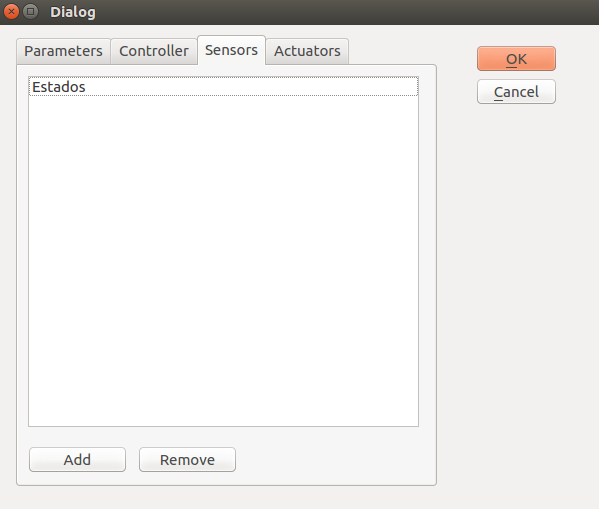
\includegraphics[width=230pt]{figuras/6.png}}
	\hfill
	\subfloat{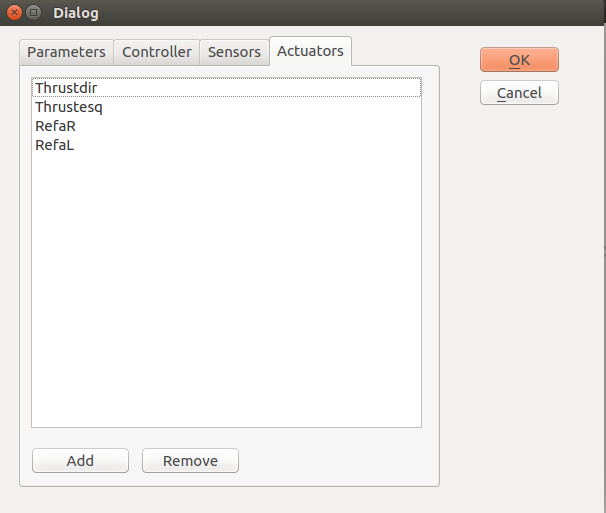
\includegraphics[width=230pt]{figuras/7.png}}
	\hfill
	\caption{Abas Sensors e Actuators.}
	\label{abas}
\end{figure}

Neste exemplo, o controlador receberá um vetor de sensores, no entanto contendo informações fornecidas por um único sensor, cujo tópico de comunicação é denominado ''Estados''. Além disso, o controlador deverá  retornar um vetor de ponto flutuante de dimensão 4 com sinais de entrada de controle para atuadores, cujos tópicos de comunicação estão na seguinte ordem: 1) Thrustdir, 2) Thrustesq, 3) RefaR e 4) RefaL.

\subsection{Criando uma nova estratégia de controle}

Para criar uma nova estratégia de controle, na aba Controller, pressione ''New Controller''. Uma nova janela será mostrada solicitando ao usuário o nome do novo controlador. Neste exemplo, a estratégia de controle terá o nome ''vant2load\_hinfinity'' (Figura \ref{projeto1}). Depois de confirmar o nome do controlador, uma janela do Nautilus aparecerá com o diretório do projeto criado (Figura \ref{2a}).

\begin{figure*}[!ht]
	\centering
	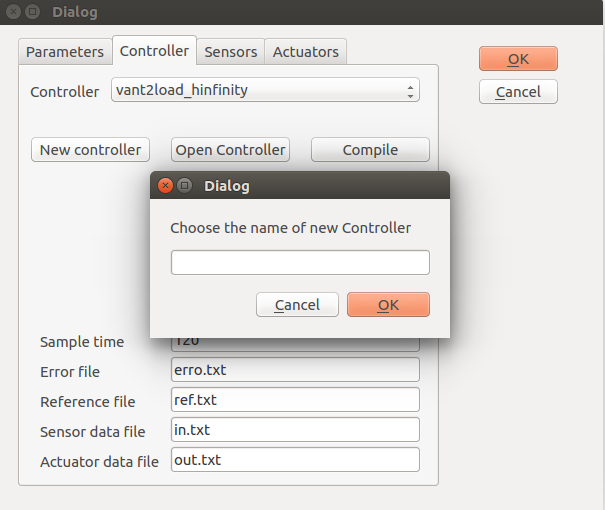
\includegraphics[width=0.7\columnwidth]{figuras/1a1a1.png}
	\caption{Criando uma nova estratégia de controle.}
	\label{projeto1}
\end{figure*}

\begin{figure*}[!ht]
	\centering
	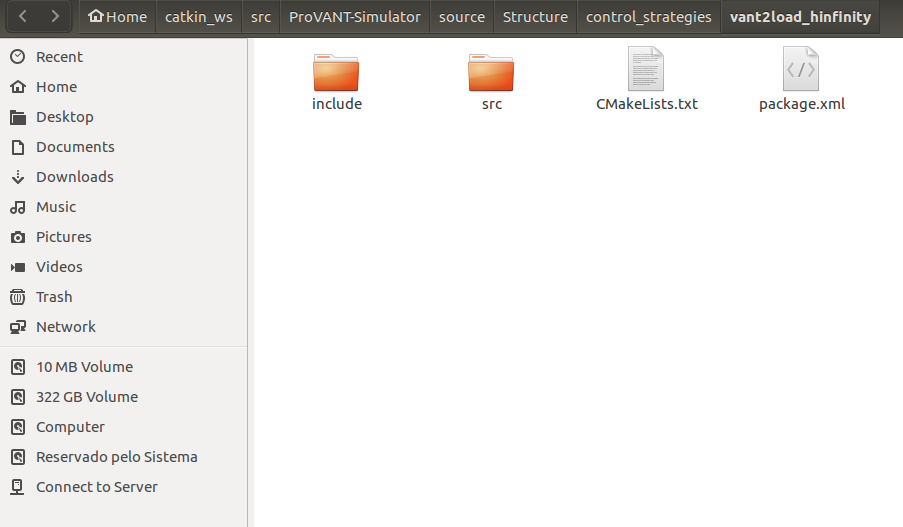
\includegraphics[width=0.7\columnwidth]{figuras/2a.png}
	\caption{Arquivos e diretórios associados à nova estratégia de controle.}
	\label{2a}
\end{figure*}

\subsection{Implementação da estratégia de controle}

A Figura \ref{exemplo1} mostra um exemplo de código de estratégia de controle implementada no arquivo main.cpp. No exemplo, observa-se que é necessário a inclusão de 3 bibliotecas: 

\begin{figure}
\begin{minted}{cpp}
#include "Icontroller.hpp"
#include <Eigen/Eigen>
#include "simulator_msgs/Sensor.h"
	
class hinfinity : public Icontroller 
{
	private: Eigen::VectorXd Xref; // vetor de referência
	private: Eigen::VectorXd Erro; // vetor de erros
	private: Eigen::VectorXd Input; // sinais de controle
	private: Eigen::MatrixXd K; // matriz de ganhos do controlador
	private: Eigen::VectorXd X; // vetor de estados
	private: double T; // Período de amostragem
	
	public: hinfinity(): Xref(24), K(4,24), X(24), Erro(24), Input(4)
	{ 
		T = 0.012;
	}
	public: ~hinfinity(){	}
	
	public: void config()
	{	
		K<< [...] Dados da matriz [...];
	}
	public: std::vector<double> execute(simulator_msgs::SensorArray arraymsg)
	{
		static float count = 0;
		static float xint, x_ant = 0;
		static float yint, y_ant = 0;
		static float zint, z_ant = 0;
		static float yawint, yaw_ant = 0;
		// selecionando dados
		int i = 0;		
		simulator_msgs::Sensor msgstates;
		msgstates = arraymsg.values.at(0);		
		// Referência
		float trajectoryRadius = 2;
		float trajectoryHeight = 4*trajectoryRadius;
		float trajTime = 80;
		float pi = 3.14;
		float x = trajectoryRadius*cos((count*T)*2*pi/trajTime);
		float xdot = -trajectoryRadius*(2*pi/trajTime)*sin((count*T)*2*pi/trajTime);
		float xddot = -trajectoryRadius*(2*pi/trajTime)*(2*pi/trajTime)
				*cos((count*T)*2*pi/trajTime);
		float y = trajectoryRadius*sin((count*T)*2*pi/trajTime);
		float ydot = trajectoryRadius*(2*pi/trajTime)*cos((count*T)*2*pi/trajTime);
		float yddot = -trajectoryRadius*(2*pi/trajTime)*(2*pi/trajTime)
				*sin((count*T)*2*pi/trajTime);
		float z = trajectoryHeight+1 - trajectoryHeight*cos((count*T)*2*pi/trajTime);
		float zdot = trajectoryHeight*(2*pi/trajTime)*sin((count*T)*2*pi/trajTime);
		float zddot = trajectoryHeight*(2*pi/trajTime)*(2*pi/trajTime)
				*cos((count*T)*2*pi/trajTime);
		Xref << x,y,z,0,0,0,0.00002965,0.004885,0.004893,0.00484,xdot,ydot,zdot,
			0,0,0,0,0,0,0,0,0,0,0;
		
		\end{minted}
		\end{figure}
		\begin{figure}
		\begin{minted}{cpp}
		//Convertendo velocidade angular
		std::vector<double> etadot = pqr2EtaDot(msgstates.values.at(13),
		msgstates.values.at(14),
		msgstates.values.at(15),
		msgstates.values.at(3),
		msgstates.values.at(4),
		msgstates.values.at(5));
		
		// Integrador Trapezoidal
		float x_atual = msgstates.values.at(0) - Xref(0);
		xint = xint + (T/2)*(x_atual + x_ant);
		x_ant = x_atual;
		float y_atual = msgstates.values.at(1) - Xref(1);
		yint = yint + (T/2)*(y_atual + y_ant);
		y_ant = y_atual;
		float z_atual = msgstates.values.at(2) - Xref(2);
		zint = zint + (T/2)*(z_atual + z_ant);
		z_ant = z_atual;
		float yaw_atual = msgstates.values.at(5) - Xref(5);
		yawint = yawint + (T/2)*(yaw_atual + yaw_ant);
		yaw_ant = yaw_atual;
		
		// vetor de estados aumentado
		X << msgstates.values.at(0),//x
		msgstates.values.at(1),//y
		msgstates.values.at(2),//z
		msgstates.values.at(3),//roll
		msgstates.values.at(4),//pitch
		msgstates.values.at(5),//yaw
		msgstates.values.at(8),//g1 x
		msgstates.values.at(9),//g2 y
		msgstates.values.at(6),//aR
		msgstates.values.at(7),//aL
		msgstates.values.at(10),//vx
		msgstates.values.at(11),//vy
		msgstates.values.at(12),//vz
		etadot.at(0),//droll
		etadot.at(1),//dpitch
		etadot.at(2),//dyaw
		msgstates.values.at(18), // angulo da primeira junta da carga
		msgstates.values.at(19), // angulo da segunda junta da carga
		msgstates.values.at(16), // derivada do angulo da primeira junta da carga
		msgstates.values.at(17), // derivada do angulo da segunda junta da carga
		xint,
		yint,
		zint,
		yawint;
		
		
		// lei de controle
		Erro = X-Xref;
		Input = -K*Erro;
		
		\end{minted}
		\end{figure}
		\begin{figure}
		\begin{minted}{cpp}
		
		// Criando vetor com dados da trajetória de referência
		Eigen::MatrixXd qref(10,1);
		qref << x,y,z,0,0,0,0.00002965,0.004885,0.004893,0.00484;
		Eigen::MatrixXd qrefdot(10,1);
		qrefdot << xdot,ydot,zdot,0,0,0,0,0,0,0;
		Eigen::MatrixXd qrefddot(10,1);
		qrefddot << xddot,yddot,zddot,0,0,0,0,0,0,0;
		
		// Feedforward
		Input(0) = Input(0) + 12.6005;
		Input(1) = Input(1) + 12.609;
		count++; 
		
		
		// convertendo dados do vetor da biblioteca Eigen para vetor a biblioteca padrão de C++
		std::vector<float> out2(Input.data(), Input.data() + Input.rows() 
					* Input.cols());
		
		std::vector<double> out(out2.size());
		for(int i=0; i<out2.size();i++) out.at(i) = out2.at(i);
		return out;
	}
	
	public: std::vector<double> Reference()
	{
		std::vector<double> out(Xref.data(), Xref.data() + Xref.rows() 
					* Xref.cols());
		return out;
	}
	
	public: std::vector<double> Error()
	{
		std::vector<double> out(Erro.data(), Erro.data() + Erro.rows() 
					* Erro.cols());	
		return out;
	}	
	
	public: std::vector<double> State()
	{
		std::vector<double> out(X.data(), X.data() + X.rows() * X.cols());
		return out;
	}
	
	private: std::vector<double> pqr2EtaDot(double in_a, double in_b, double in_c, 
						double phi, double theta, double psii)
	{
		std::vector<double> out;
		out.push_back(in_a + in_c*cos(phi)*tan(theta) + in_b*sin(phi)*tan(theta));
		out.push_back(in_b*cos(phi) - in_c*sin(phi));
		out.push_back((in_c*cos(phi))/cos(theta) + (in_b*sin(phi))/cos(theta));
		return out;
	}
};
	
	\end{minted}
	\end{figure}
	\begin{figure}
	\begin{minted}{cpp}
	
extern "C"
{ 
	Icontroller *create(void) {
		return new hinfinity;
	}
	void destroy(Icontroller *p) {
		delete p;
	}
}
\end{minted}
\caption{Exemplo de código.}
\label{exemplo1}
\end{figure}

\begin{itemize}
		\setlength{\itemsep}{1pt}
		\setlength{\parskip}{0pt}
		\setlength{\parsep}{0pt}
\item \#include ''Icontroller.hpp''  - informa ao código a interface padrão para criação de controladores no ambiente de simulação;
\item \#include <Eigen/Eigen> - importa as funcionalidades fornecidas pela biblioteca Eigen \footnote{https://eigen.tuxfamily.org}. A biblioteca Eigen fornecer funções para realizar operações da álgebra linear;
\item \#include ''simulator\_msgs/Sensor.h'' - informa a classe responsável por abstrair o padrão de comunicação entre o controlador e os sensores.
\end{itemize}


Os atributos \textbf{Xref}, \textbf{Erro}, \textbf{Input}, \textbf{K} e \textbf{X} são as estruturas de de vetores e matrizes da biblioteca Eigen. Essas estruturas são responsáveis por realizar a operações de álgebra linear e, portanto, permitir a relização da lei de controle. O atributo \textbf{T} determina o período de amostragem do controlador.

O construtor hinfinity() inicializa os atributos da classe, enquanto o destrutor \textasciitilde hinfinity() não possui nenhuma função no contexto do simulador.

Neste exemplo, o método config() é utilizado para atribuir valores à matriz de ganhos K, respeitando a sintaxe da biblioteca Eigen, no entanto o usuário pode utilizar esse espaço para realizar qualquer outra configuração inicial. Por fim, a lógica da estratégia de controle é implementada no método execute(), que é executado a cada período de amostragem, como descrito anteriormente.

O código começa por declarar as variáveis (estáticas) ''xint'', ''x\_ant'', ''yint'', ''y\_ant'', ''zint'', ''z\_ant'', ''yawint'' e ''yaw\_ant'', utilizadas para armazenar os valores dos integradores implementados na estratégia de controle. Em seguida, está presente o trecho de código referente aos dados dos sensores, obtidos através do vetor ''arraymsg''. Como neste exemplo somente um sensor está disponível (''Estados''), apenas a primeira posição deste vetor é acessada (através da sintaxe ''arraymsg.values.at(0)''). Nos casos em que mais sensores são disponibilizados, os dados do n-ésimo sensor são acessados através de  ''arraymsg.values.at(n-1)'' e a ordem desse vetor é definida a priori na aba Sensor conforme é visualizada em \ref{6}. Em seguida, é definido a referência para o controlador e implementado integradores, através do método de integração trapezoidal, para realização da lei de controle e, por fim, é calculada a ação de controle feedforward. 

Os métodos Reference(), Error(), State() são utilizados para armazenar dos sinais de referência, erro e estados, respectivamente, nos arquivos de texto de saída do ambiente de simulação. A função pqr2EtaDot() corresponde a um mapeamento de parte das informações recebidas pelos sensores, necessário para a implementação da estratégia de controle deste exemplo. 

Assim como a função pqr2EtaDot(), quaisquer funções adicionais que sejam necessárias para a implementação da estratégia de controle, podendo estar relacionadas também a algoritmos de filtragem, podem ser escritas dentro da classe ''main.cpp'', ou em classes auxiliares criadas dentro da pasta ''include'' ilustrada em \ref{2a} (neste caso, estas devem ser também incluídas no cabeçalho do arquivo ''main.cpp'').


Por fim, o trecho de código a seguir corresponde à funções necessárias para garantir o carregamento da estratégia de controle em tempo de execução do simulador. O método create() cria uma instância da classe que encapsula o controlador, e o método destroy() é utilizado para destruir a instância da classe.

\begin{minted}{cpp}
extern "C"
{ 
	Icontroller *create(void) {
		return new hinfinity;
	}
	void destroy(Icontroller *p) {
		delete p;
	}
}
\end{minted}


%\subsection{Configurando CMakeLists.txt}
%
%Em seguida, substitua o código template do CMakeLists.txt com o seguinte código.
%
%
%\begin{minted}{xml}
%cmake_minimum_required(VERSION 2.8.3)
%project(vant2load_hinfinity)
%
%find_package(catkin REQUIRED COMPONENTS
%			roscpp
%			simulator_msgs)
%	
%include_directories(include)
%INCLUDE_DIRECTORIES (/usr/include/eigen3)
%include_directories( ${catkin_INCLUDE_DIRS})
%include_directories($ENV{TILT_PROJECT}/source/Structure/control_strategies/)
%
%add_library(vant2load_hinfinity src/hinfinity.cpp)
%target_link_libraries(vant2load_hinfinity ${catkin_LIBRARIES})
%install(TARGETS
%vant2load_hinfinity
%ARCHIVE DESTINATION ${CATKIN_PACKAGE_LIB_DESTINATION}
%LIBRARY DESTINATION ${CATKIN_PACKAGE_LIB_DESTINATION}
%RUNTIME DESTINATION ${CATKIN_PACKAGE_BIN_DESTINATION})
%\end{minted}
%
%
%\subsection{Configurando package.xml}
%
%Em seguida, substitua o código template do package.xml com o seguinte código.
%
%\begin{minted}{xml}
%<?xml version="1.0"?>
%<package>
%	<name>vant2load_hinfinity</name>
%	<version>1.0.0</version>
%	<description>The hinfinity package</description>
%	
%	<maintainer email="macro@todo.todo">macro</maintainer>
%	<license>TODO</license>
%	
%	<buildtool_depend>catkin</buildtool_depend>
%	<build_depend>roscpp</build_depend>
%	<run_depend>roscpp</run_depend>
%	<build_depend>simulator_msgs</build_depend>
%	<run_depend>simulator_msgs</run_depend>
%	
%	<export>
%	</export>
%
%</package>
%\end{minted}
%
%O arquivo package.xml deste exemplo informa que o nome do pacote que encapsula o projeto de controle é denominada de "vant2load_hinfinity"

\subsection{Compilando o código da estratégia de controle}

Após a implementação da estratégia de controle, o código correspondente pode ser compilado através do botão ''Compile'' (conforme explicado no Capítulo 2, vide Figura \ref{5}, item 4).

%\chapter{Inserção de novo cenário}
%
%Um cenário no Gazebo é uma instância de simulação composto por um ou mais modelos incluídos. Este ambiente de simulação está formatado para o funcionamento de apenas um VANT, sendo que demais modelos incluídos são ilustrativos. Há duas maneiras de se incluir um novo cenário: cenário template e cenário editável e pronto para simular. 
%
%O cenário template é a criação de um arquivo com sufixo ".tpl" que tenha apenas elementos ilustrativos e não seja editável pela interface gráfica de configuração. Já o outro é um cenário pronto para uso com VANT definido com sufixo ".world". A estrutura organizacional de ambos os cenários está ilustrado a seguir:
%
%
%\begin{lstlisting}
%<?xml version="1.0" encoding="UTF-8"?>
%<sdf version="1.6">
%	<world name="/home/macro/catkin_ws/src/provant_simulator/source/Database/simulation_elements/worlds/templates/empty/empty2.tpl">
%		<gravity>0.000000 0.000000 -9.8000</gravity>
%		<physics type="ode">
%			<max_step_size>0.001000</max_step_size>
%			<real_time_factor>0</real_time_factor>
%		</physics>
%		<plugin name="gazebo_tutorials" filename="libgazebo_ros_world_plugin.so"/>
%		<include>
%			<uri>model://ground_plane</uri>
%			<static>false</static>
%		</include>
%		<include>
%			<uri>model://sun</uri>
%			<static>false</static>
%		</include>
%		<include>
%			<uri>model://vant_2.0</uri>
%			<name>newmodel</name>
%			<static>false</static>
%			<pose>0 0 2 0 0 0</pose>
%		</include>
%		<scene>
%			<sky>
%				<time>18</time>
%				<clouds>
%					<speed>0</speed>
%				</clouds>
%			</sky>
%		</scene>
%	</world>
%</sdf>
%\end{lstlisting}
%
%onde,
%
%\begin{itemize}
%	\setlength{\itemsep}{1pt}
%	\setlength{\parskip}{0pt}
%	\setlength{\parsep}{0pt}
%	\item[-] <gravity></gravity> valores de definição do vetor de aceleração da gravidade (em $metros/s^2$).
%	\item[-] atributo "type" da tag physics : especifica qual motor de simulação será utilizado 
%	\item[-] <physics><max\_step\_size></max\_step\_size></physics> valor do passo de simulação (em milissegundos)
%	\item[-] <physics><real\_time\_factor><real\_time\_factor></max\_step\_size><physics> valor 1 define que o Gazebo tentará funcionará em tempo real e 0 define que o Gazebo funcionará o mais rápido possível. 
%	\item[-] <plugin></plugin> definição do plugin mundo com a função de sincronização da simulação;
%	\item[-] <include><uri></uri></include> nome do modelo a ser incluído no cenário
%	\item[-] <include><static></static></include> define se o modelo terá dinâmica simulada pelo motor de simulação
%	\item[-] <include><name></name></include> nome do modelo
%	\item[-] <include><pose></pose></include> pose inicial do modelo na simulação
%	\item[-] <scene><time></time></scene> hora do dia q a simulação simulará
%	\item[-] <scene><clouds><speed></speed></clouds></scene> inclusão de nuvens na simulação e sua respectiva velocidade
%\end{itemize}
%
%Obs.: Esta versão do ambiente de simulação está preparado para receber apenas essas configurações. Não adicione outros tipos de informação. 
%  
%


%

%
%\chapter{Arquitetura de software}
%
%\section{Malha de controle}
%
%A malha de controle desenvolvida neste trabalho está ilustrada na Figura x e é composta por um nó Controlador. O nó Controlador é o local obtém as informações sensoriais, coloca na ordem pre-definida pelo usuário, executa a lei de controle e envia os sinais de controle para o simulador. Assim que o modelo recebe os novos comandos, é realizado um novo passo de simulação, fechando o laço de comunicação.
%
%\begin{figure}[!htb]
%	%\vspace{-3mm}
%	\centering{
%		\def\svgwidth{0.745\columnwidth}
%		%{\footnotesize\import{Figuras/}{simulator_flowchart.pdf_tex}}%\vspace{-1mm}
%		{\footnotesize\import{figuras/}{simulator_flowchartV2.pdf_tex}}%\vspace{-1mm}
%		%\caption{Fluxo de funcionamento do ambiente de simulação.}\label{flow}}%kinematics}}
%		%\caption{Estrutura do ambiente de simulação.}\label{flow}}%kinematics}}
%		\caption{Fluxo de informações do ambiente de simulação.}\label{flow}}%kinematics}}
%	%\vspace{-3mm}
%\end{figure}
%
%\section{Interface Gráfica}
%
%O código desenvolvido está organizado em três níveis de modularização: “camada de acesso a dados”, “camada de negócios” e ”camada de apresentação”. A Figura x ilustra esta organização. Esses níveis proveem facilidade de manutenção do código e desacoplamento de funcionalidades.
%
%Na “camada de acesso a dados” estão as classes responsáveis por ler e escrever em arquivos XML. Nesse nível de desenvolvimento utilizou-se o módulo de software QXml fornecida pela API do ambiente de desenvolvimento QT para ter acesso à hierarquia de informações do arquivo XML. Na “camada de negócios”, encontram-se as classes responsáveis por descrever a estrutura de dados onde são armazenados os detalhes de configuração dos modelos. Já a “camada de apresentação” define a apresentação e as funcionalidades da interface gráfica.
%
%\begin{figure*}[!ht]
%	\centering
%	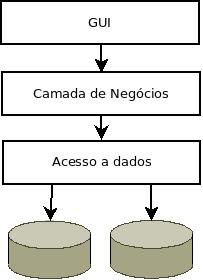
\includegraphics[width=100pt]{figuras/threelayers.jpeg}
%	\caption{Arquitetura de software da interface gráfica}
%	\label{7}
%\end{figure*}
%
%%\appendix
%
%%\chapter{ROS}